\section{Fazit}
\label{sec:fazit}

%Das Ziel dieser Arbeit, das Agentenkonzept für die realistische Verkehrssimulation nutzen zu können, konnte erreicht werden.
Anders als bei den Simulationen zur ursprünglichen Arbeit von Nagel und Schreckenberg \cite{na-sch} findet bei den Simulationen mit dem Agentenkonzept %eine Simulation von Verkehr mit Werten durchgeführt werden, die ähnlich den real auftretenden sind.
die Interaktionen zwischen den Agenten/Fahrzeugen ausschließlich aufgrund von Größen wie Abstand, (relativer) Geschwindigkeit und relativer Position statt.
Dies ist vergleichbar zur Situation im realen Straßenverkehr.

\begin{figure}[hptb]
 \centering
 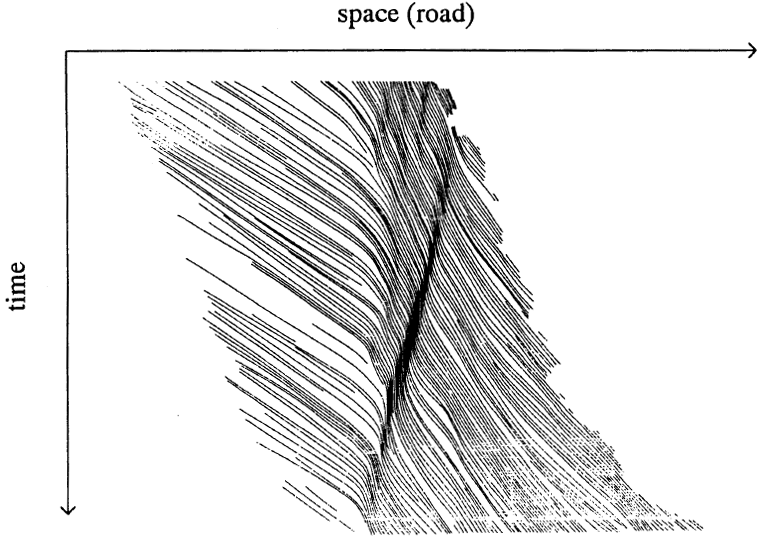
\includegraphics[width=0.65\textwidth]{welle-nasch}
 \caption[Fahrzeugbewegung in Weg-Zeit-Linien aus Luftaufnahmen]
 		{Fahrzeugbewegung in Weg-Zeit-Linien aus Luftaufnahmen, aus \cite[Fig. 3]{na-sch}}
 \label{figure:welle-nasch}
\end{figure}

Trotz dieser Veränderungen ergeben sich z.B. in der zweiten Hälfte der Simulation in \cref{figure:33veh-1km} vergleichbare Muster zu Weg-Zeit-Linien von Fahrzeugen, siehe \cref{figure:welle-nasch}, die aus Luftausnahmen gewonnen wurden.

Die Gridumgebung dient ausschließlich als Darstellung der Straße.
\\
Die Fahrspuren sind, auch bei Mehrspurigkeit, anders als bei \cite{multi-fuzzy}, keine miteinander kommunizierenden Automaten, sondern die Zellen darauf \enquote{Verankerungspunkte} für die Fahrzeuge.
Zwischen den Fahrspuren kann hin und her gewechselt werden.
Die Verantwortung für die Einhaltung von Vorgaben liegt bei jedem Agenten.
\\
Die Zellgröße wurde gegenüber dem ursprünglichen Nagel-Schreckenberg-Modell verkleinert.
Eine weitere Verkleinerung scheint möglich, wenn die Inkonsistenzen in den Beliefbases abgestellt werden können.

Die Kollisionsfreiheit des Originalmodells konnte bei zu großen Geschwindigkeitsunterschieden nicht dargestellt werden.
Dadurch dass die Auslösung des Kollisionsereignisses bereits bei Unterschreitung eines Mindestabstandes stattfindet, der abhängig von der aktuell gefahrenen Geschwindigkeit ist, gelang es ebenfalls nicht, eine realistische Unfallhäufigkeit zu erreichen.
Ebenso wurde die Möglichkeit einer engen Fahrzeugfolge dadurch beeinflusst.

Bei der Verkehrsfluss/Verkehrsdichte-Ebene des Fundamentaldiagrammes gelang nur die Darstellung des aufsteigenden Astes, die frei fließenden Verkehr bedeutet.



%%%%%%%%%%%%%%%%%%%%%%%%%%%%%%%%%%%%%%%%%%%%%%%%%%%%%%%%%%%
%	NEW SUBSECTION
%%%%%%%%%%%%%%%%%%%%%%%%%%%%%%%%%%%%%%%%%%%%%%%%%%%%%%%%%%%



\subsection{Ausblick}
\label{sec:ausblick}

Durch eine weitere Reduzierung der Größe der Gridzellen und Verkleinerung der Zeitschritte ist die Diskretisierung der Simulationsumgebung möglich.
Problematisch ist hier allerdings die aktuelle Entstehung von Inkonsistenzen in den Entscheidungsgrundlagen der Agenten zu sehen.

Durch die Verkleinerung der Zellgröße wird es nötig sein, dass für Fahrzeuge bei der Initialisierung eine Fahrzeuglänge generiert wird.
Diese würden dann mehrere dieser dann kleineren Zellen überdecken.
Folge wäre ein diversifizierteres Fahrzeugbild (Fahrzeugklassen), das auch in Sachen Platzbedarf realistisch dargestellt werden kann.

Für die Zukunft muss ein Weg gefunden werden, die Fahrzeuge innerhalb real möglicher Abstände so abzubremsen, dass keine Kollisionen entstehen. 
%Es sollte ein Weg gefunden werden, die Bremskräfte zu dosieren. 
%Wie in den Überlegunden für die Pull-out-Wahrscheinlichkeit (\cref{sec:pullout-pullin}) gezeigt, könnte sich auch hierfür eine Kombination aus Abstand und relativer Geschwindigkeit eignen.

Wenn es die Weiterentwicklung von \enquote{LightJason} zulässt, sollte mit den in \cref{sec:ueberlegungen-multilane} getätigten Überlegungen geprüft werden, ob die Mehrspurversion des Agentenscriptes unter Belastung eingesetzt werden kann.

Das Agentenmodell selbst kann ebenfalls noch um Komponenten der Realität erweitert werden.

\paragraph*{Fahrertypen}
\hfill \\
Im Jahr 2015 wurde bei einer Studie der London School of Economics and Political Science (LSE) im Auftrag des Reifenherstellers Goodyear, siehe \cite{fahrertyp}, festgestellt, dass man Autofahrer in sieben Typen einteilen kann.
\begin{itemize}
\itemsep0em
	\item \enquote{the teacher}, der Lehrer: möchte, dass andere Fahrer wissen, was sie falsch gemacht haben und erwartet Anerkennung für seine Anstrengungen andere zu belehren
	\item \enquote{the Know-it-all}, der Besserwisser: denkt, dass er von inkompetenten Schwachköpfen umgeben ist und schreit diese gelegentlich auch schon einmal an, während er sicher in seinem Auto sitzt
	\item \enquote{the Competitor}, der Wettkämpfer: muss vor allen anderen Fahrern sein und reagiert verärgert, wenn sich diesem Ziel jemand entgegen stellt, beschleunigt evtl. falls jemand zu überholen versucht oder schließt die Lücke um ein Einfädeln unmöglich zu machen
	\item \enquote{the Punisher}, der Bestrafer: möchte jeden anderen Fahrer für gefühltes Fehlverhalten bestrafen, steigt ggf. aus dem Auto aus, um andere Fahrer direkt zu konfrontieren
	\item \enquote{the Philosopher}, der Philosophische: akzeptiert Fehlverhalten problemlos und versucht dieses rational zu erklären, versteht es seine Gefühle im Auto zu kontrollieren
	\item \enquote{the Avoider}, der Vermeider: behandelt Fahrer, die sich daneben benehmen, unpersönlich, tut sie als Gefahr ab
	\item \enquote{the Escapee}, der Flüchter: hört Musik oder spricht am Telefon, um sich zu isolieren, lenkt sich mit ausgewählten sozialen Beziehungen ab, um sich nicht mit anderen Fahrern auf der Straße beschäftigen zu müssen, in erster Linie ist es aber eine Strategie, das Aufkommen von Frust zu vermeiden
\end{itemize}

Für zukünftige Entwicklungen der Simulation könnte man für diese oder ähnliche Fahrertypen Profile ausarbeiten und anlegen, die sich auf Abstands-, Beschleunigungs- und Ver"-zö"-ge"-rungs"-ver"-hal"-ten sowie die Risikobereitschaft beim Aus- und Einscheren auswirken.
So könnte noch eine weitere Komponente mit Hinsicht auf Realitätsnähe geschaffen werden. 

\paragraph*{Stresslevel}
\hfill \\
Weiterhin könnte \enquote{Hupen} als Broadcast- oder Message-Ereignis festgelegt werden.
Dies oder auch wiederholtes zu dichtes Auffahren und \enquote{geschnitten werden}, könnten sich auf eine Art Stresslevel auswirken, das als interner Belief im Agenten hinterlegt wird.
\\
Das Stresslevel wiederum könnte die Art und Weise verändern, wie das jeweilige Fahrzeug am Straßenverkehr teilnimmt. 
Ggf. auch in unterschiedlicher Art und Weise, je nach Fahrertyp.
\\
Über eine gewisse Zeit, baut sich erworbener Stress wieder ab.

\paragraph*{Außenwahrnehmung der Fahrzeuge}
\hfill \\
Die Außenwahrnehmung eines Fahrzeuges könnte durch einen öffentlich sichtbaren Belief gesteuert werden. 

Ist ein Fahrer betrunken, fällt dies anderen Fahrern normalerweise u.a. aufgrund der Fahrweise auf.
Hier könnte z.B. der Hinweis, dass der Fahrer betrunken ist, andere Fahrzeuge vorsichtiger handeln lassen.

Ein weiterer Aspekt könnte die Fahrtrichtungsanzeige sein.
Blinkt ein Fahrzeug, um einen Spurwechsel anzuzeigen, wird ein nachfolgender Fahrer evtl. nicht weiter beschleunigen. 



%%%%%%%%%%%%%%%%%%%%%%%%%%%%%%%%%%%%%%%%%%%%%%%%%%%%%%%%%%%
%	NEW SUBSECTION
%%%%%%%%%%%%%%%%%%%%%%%%%%%%%%%%%%%%%%%%%%%%%%%%%%%%%%%%%%%


\subsection{Das NaSch-Modell in der Zukunft}
Wird das Nagel-Schreckenberg-Modell zukünftig noch von Bedeutung sein? 
Viele Entwicklungen im Automobilbereich gehen aktuell in Richtung hochassitentes oder gar autonomes Fahren.
Wie wird man diese Art der individuellen Fortbewegung simulieren können?

Laut \cite{automation-level} kann neben dem manuellen Fahren in fünf Stufen der Automation unterschieden werden.
Zur Zeit befindet man sich am Übergang von Stufe 2 zu Stufe 3, ab der die Umwelt automatisiert überwacht wird.
Dies findet durch sog. Assistenzsysteme statt.
Diese können den Fahrer unterstützen - Notbremsassistenten, Spurhalteassistenten - entbinden diesen aber nicht von seiner eigenen Sorgfaltspflicht.
Zudem ist etwa ein Abbremsen eines Assistenzsystems abrupt und wesentlich stärker als das eines Menschen.
Somit käme man wesentlich eher an den Punkt, an dem ein Fahrzeug so stark abbremsen muss, dass es still steht.

Bei aktuell erhältlichen, serienmäßigen Fahrzeugen ist - zumindest durch die Gesetzgebung - immer noch ein menschlicher Fahrer nötig.
Selbst die Firma Tesla, die das eigene \enquote{Autopilot}-System auf ihrer Webseite mit \enquote{Full Self-Driving Capability}/\enquote{Volles Potenzial für autonomes Fahren} anpreist (vgl. \cite{tesla-en} und \cite{tesla-de}), verweist in der eigenen Internetpräsentation und bei Reaktionen auf Unfälle mit ihren Fahrzeugen darauf, dass der Fahrer selbst auf die Straße achten muss. \cite{firetruck-accident}
%\footnote{siehe \url{https://www.tesla.com/autopilot}, abgerufen am 18. März 2018}
%\footnote{siehe \url{https://www.tesla.com/de_DE/autopilot}, abgerufen am 18. März 2018} 
%\footnote{siehe \url{http://money.cnn.com/2018/01/23/technology/tesla-fire-truck-crash/index.html}, abgerufen am 18. März 2018}.

Sollten diese Systeme in der Zukunft zu 100\% sicher funktionieren und gesetzlich erlaubt werden, kann man den Faktor Mensch, der meist die Unsicherheiten in das System Verkehr einbringt, aus der Gleichung entfernen.
Von diesem Punkt ist die Technik aktuell noch ein Stück weit entfernt (vgl. \cite{how-far-is-autonomous-driving}), sodass der Mensch hinter dem Lenkrad wohl noch einige Zeit erhalten bleiben wird \ldots\hspace{0.05em} und sei es als Backup bei Fehleinschätzungen der Technik.
%\footnote{siehe \url{http://www.sueddeutsche.de/auto/verkehrssicherheit-so-weit-ist-das-autonome-fahren-1.3913983}, abgerufen am 20. März 2018}
Somit hat das Nagel-Schreckenberg-Modell auch zukünftig seine Berechtigung.

Und selbst im Falle der vollständigen Automation gelten für die Fahrzeuge die gleichen physikalischen Voraussetzungen.
Da die Straßenfahrzeuge nicht untereinander gekoppelt werden, sind gewisse Verzögerungen und Abweichungen der Reaktionen nach wie vor vorhanden.
\\
Wichtig wäre die Kommunikation der Fahrzeuge untereinander.
Dann könnten Verzögerungen durch Reaktionszeiten ggf. noch weiter gesenkt werden.
